\chapter{A Private Cloud for MapReduce Applications}\label{cap:solucion}
\noindent This chapter introduces a novel solution combining the virtual infrastructure managed with OpenStack and the Hadoop implementation of MapReduce to conform a powerful computational tandem. \emph{qosh}, as this project has been called, will be described along this section moving from architecture to implementation.

\section{Architecture}\label{sec:diseno}
\noindent Figure \ref{fig:arquitecturaglobal} shows a high level portrait of qosh execution environment. The component that acts as interface between system and user is displayed on the right end. It abstracts the inherent difficulty in configuring the job execution context and in deploying the virtual cluster. Furthermore, qosh will keep track of submitted jobs, MapReduce \texttt{jar} files, input data and output results, with no need to walk the HDFS to search for data.

\begin{figure}[tbp]
\begin{center}
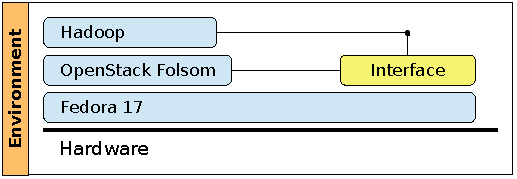
\includegraphics[width=0.65\textwidth]{imagenes/021.pdf}
 \caption{Global Architecture}
\label{fig:arquitecturaglobal}
\end{center}
\end{figure}

To streamline development, it is determined that the very first qosh version be tested on a personal computer. As shown on figure \ref{fig:arquitecturaglobal}, Fedora Linux is installed atop the hardware and OpenStack Folsom set up within. qosh will draw on the infrastructure provided by the local OpenStack configuration to deploy virtual Hadoop clusters. While it would be better to make qosh more flexible allowing for remote infrastructure consumption, it would also become harder to test.

Figure \ref{fig:arquitecturadetalle} shows a more detailed view on qosh design details. The VM contains a Hadoop installation ready to be put to use as soon as it was started. The VM life cycle is managed by OpenStack and its execution environment shaped by KVM, the chosen hypervisor. Besides, HDFS has been used as temporal persistence layer while the results are not send back to the controller --- the same machine in this testing environment. It shall be recalled that even though HDFS is a steady data store, the Hadoop VMs are created and removed for every workflow execution effectively destroying HDFS data at the end of processing each job. So, it is qosh's job to orchestrate data extraction before shutting down the virtual cluster.

\begin{figure}[tbp]
\begin{center}
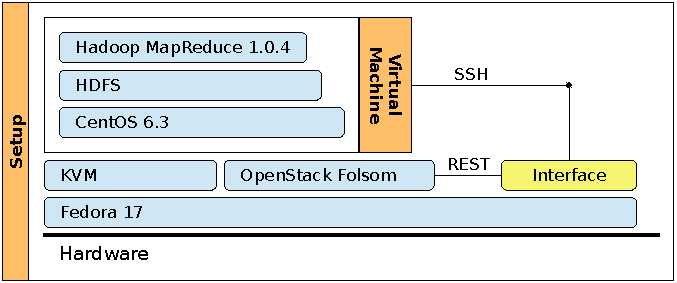
\includegraphics[width=0.85\textwidth]{imagenes/022.pdf}
 \caption{Detailed global architecture}
\label{fig:arquitecturadetalle}
\end{center}
\end{figure}

Figure \ref{fig:arquitecturainterfaz} shows the modular decomposition of qosh orchestration module.

\begin{figure}[bp]
\begin{center}
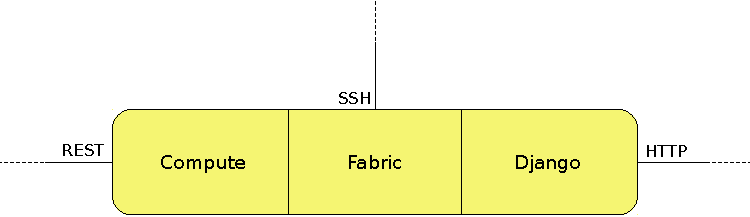
\includegraphics[width=0.8\textwidth]{imagenes/023.pdf}
 \caption{Core qosh modular decomposition}
\label{fig:arquitecturainterfaz}
\end{center}
\end{figure}

\begin{description}
 \item[Compute:] Acts as client to OpenStack REST API. It handles every interaction with the cloud decoupling qosh fromt the particular IaaS Cloud.
 \item[Django:] Is used in qosh to let users manage their MapReduce executions with ease via a web interface.
 \item[Fabric:] Is the Python library included in qosh to configure the virtual cluster deployment and destruction.
\end{description}

\subsection{Design Diagrams}\label{subsec:diagramasaltonivel}
\noindent Below are shown the design diagrams that make up the section on high level overview of the project.

\subsubsection{Django Components}\label{subsubsec:componentesdjango}
\noindent Figure \ref{fig:instalaciondjango} portrays modules adjacent to Django to support its operation.

\begin{figure}[bp]
\begin{center}
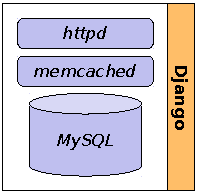
\includegraphics[width=0.23\textwidth]{imagenes/024.pdf}
 \caption{Django setup}
\label{fig:instalaciondjango}
\end{center}
\end{figure}

\begin{description}
 \item[Apache httpd:] Relied on to manage user interaction with OpenStack Dashboard, it may also be used to with qosh web interface. Initially, qosh depends on Python web server module to handle user requests, but \emph{httpd} might be easily configured.
 \item[memcached:] Is employed to cache web pages in order to speedup load times.
 \item[MySQL:] Chosen relational DBMS to store job meta-data.
\end{description}


\subsubsection{Use Cases Diagram}\label{subsubsec:casosuso}
\noindent Figure \ref{fig:casosuso} displays the set of use cases that have been considered for qosh. It reflects the five fundamental agents comprising the system.

\begin{figure}[tbp]
\begin{center}
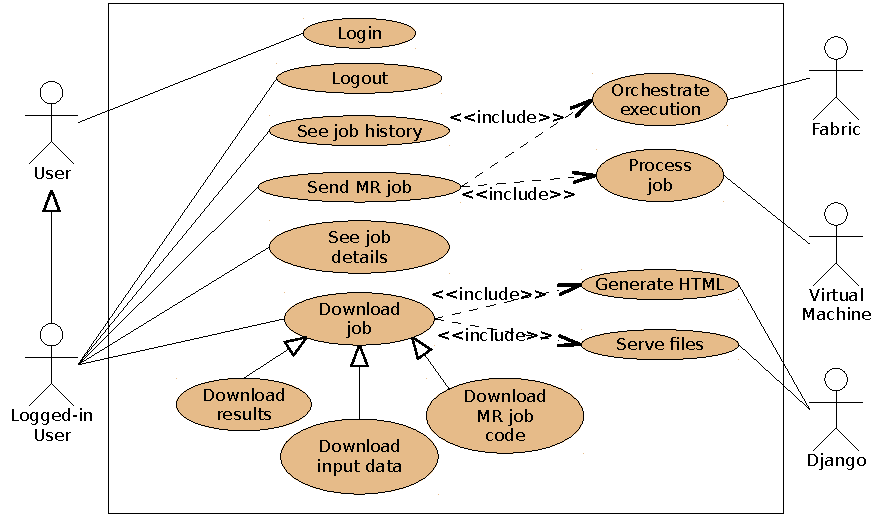
\includegraphics[width=0.99\textwidth]{imagenes/025.pdf}
 \caption{Use Cases Diagram}
\label{fig:casosuso}
\end{center}
\end{figure}

\subsubsection{Machine State Diagram}\label{subsubsec:navegacion}
\noindent Figure \ref{fig:navegacion} presents a summary on the navigation flow across the web interface. An example interaction is subsequently described.

Initially, the user is presented the \emph{Login} page so that he/she could log into qosh. If the supplied credentials were cleared --- the user must be previously registered in Keystone as user/pass is shared with qosh ---, the \emph{Main} page is shown. From there the user may \emph{Configure Job} or go over the \emph{Job History} to get some \emph{Job Details}.

\begin{figure}[tbp]
\begin{center}
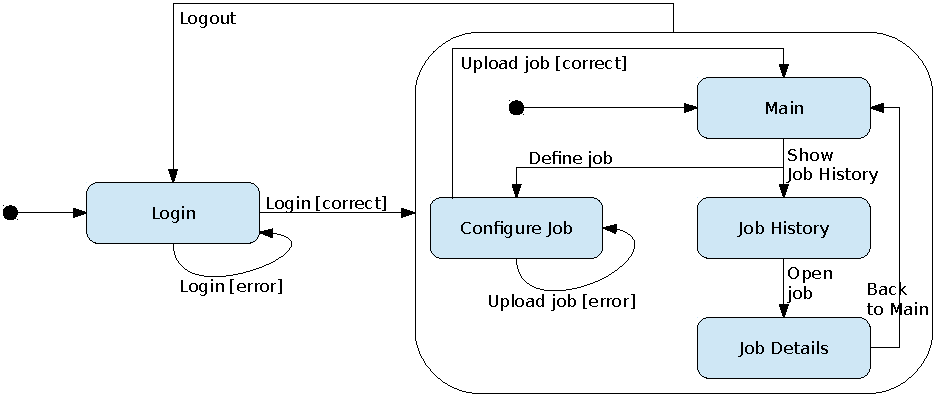
\includegraphics[width=0.99\textwidth]{imagenes/026.pdf}
 \caption{Web interface transitions}
\label{fig:navegacion}
\end{center}
\end{figure}

\subsubsection{Class Diagram --- Compute Module}\label{subsubsec:diagramaclasescompute}
\noindent Figure \ref{fig:diagramaclasescompute1} shows a small Class Diagram describing how the REST client is related to Fabric and Python.

\begin{description}
 \item[json:] Parses structured JSON-formated data and permits its manipulation. OpenStack REST API understands both XML and JSON.
 \item[Exception:] Python class representing a generic exception.
 \item[ServiceError:] Extends \texttt{Exception} to notify and handle any error that may be raised during execution. It's objects have two properties: an HTTP error code and error description.
 \item[Environment:] Contains the set of global options for configuring the virtual deployment.
 \item[httplib:] The Python module containing functions, classes and helpers toward interacting with HTTP connections. qosh banks on it to help consume the OpenStack REST service.
\end{description}

\begin{figure}[tbp]
\begin{center}
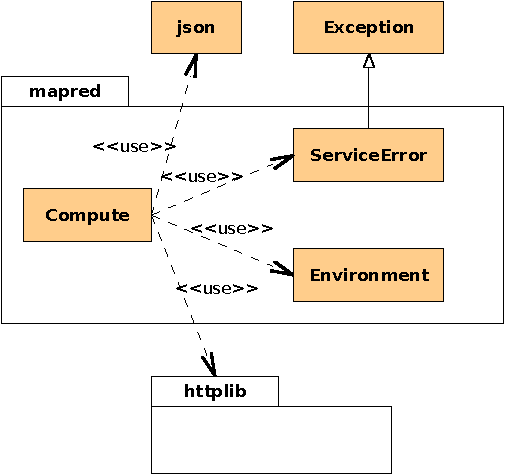
\includegraphics[width=0.5\textwidth]{imagenes/027.pdf}
 \caption{Class Diagram --- Compute module (I)}
\label{fig:diagramaclasescompute1}
\end{center}
\end{figure}

\section{Implementation}\label{sec:implementacion}
\noindent All the three modules conforming qosh core have been written in Python. The tests of the first version run over Fabric 1.4.3, Django 1.4.2 and Python 2.7.3. The configuration inside the VM is carried out by three \emph{Bash-Script}s in three different instants in the VM life cycle: before bringing the network up, after having completed the boot sequence and before shutdown. They will be detailed in section \ref{subsec:maquinavirtual}.

\subsection{Hadoop Virtual Machine}\label{subsec:maquinavirtual}
\noindent The Hadoop virtual machine is a vital asset for the qosh project; in the end it is Hadoop who executes workflows. The versions configured are Hadoop 1.0.4 and Oracle JRE 1.7. Installing and tunning every service in the VM has not been a complex process, whereas it has been long and interesting enough, for it is potentially reusable to create other customized VMs, to list every step followed to complete the setup.

\begin{itemize}
 \item In the local development machine the \emph{Virtual Machine Manager} (package \texttt{virt-manager}) was installed with \texttt{yum}. \texttt{yum} automatically installed dependent libraries like \texttt{libvirt}, the Kernel Virtual Machine hypervisor module (KVM) and a wrapper to handle it (\texttt{qemu-kvm}).
 \item Through the Virtual Machine Manager, a VM with 1 GB of RAM, 4 GB for the drive image within a \texttt{qcow2} container and both APIC and ACPI was created anew.
 \item A minimal network install of CentOS 6.3 was carried through. \emph{Basic Server} was chosen as initial package set on a single ext4 partition --- no swap partition --- without LVM.
 \item After the initial boot sequence, the distribution was put to the latest stable version available.
 \item The Oracle JRE 1.7 and Hadoop 1.0.4 were downloaded from official sources and subsequently installed on the VM.
 \item A new user (\emph{hduser}) was registered and set \emph{hadoop} as its primary group. As a result, the permission of the files related to Hadoop --- configuration files and scripts ---- were updated to allow this new user to launch and kill MapReduce jobs.
 \item \texttt{sshd} was tuned to disable superuser connections and user/pass authentication method; only ssh tunnels cleared by keypairs will be permitted.
 \item Three scripts --- similar to Ubuntu \texttt{cloud-init} scripts --- were written to \texttt{/etc/init.d/cloud-*} to customize part of the VM behavior. An important feature of them being they manage injecting the public part of the keypair used for authentication into the VM file system --- in \texttt{/home/hduser/.ssh/authorized\_keys} --- when it boots, so the owner of the private part can authenticate.
 \item The \texttt{yum groups} utility was applied to remove unused services like \emph{X-server}.
 \item From the local machine the VM was terminated and its drive image was mounted with \texttt{qemu-nbd} to remove logs and user history from the VM. Then, a 5 GB zeroed-file was created with \texttt{dd} inside the VM file system, failing, for there was not enough free space to accommodate 5 GB within a 4 GB image, while filling the remaining space up with zeros. Just after that, \texttt{qemu-img} was invoked to compress the image into a new file.
 \item Next, \texttt{fdisk} was used locally to observe the VM file system block size and initial block number of the Hadoop partition --- the only partition. By multiplying both values the partition offset was obtained, allowing for the extraction of the Hadoop partition using \texttt{qemu-nbd} offset-mounting capabilities and \texttt{dd} to dump, again, to a new file.
 \item Finally, both the \emph{initram} and the kernel image were copied out from the VM to the local file system.
\end{itemize}

\subsection{Low Level Diagrams}\label{subsec:diagramasimpl}
\noindent Next comes the diagram set that exposes those features closer to qosh implementation.

\subsubsection{Class Diagram --- Compute Module}\label{subsubsec:implementacioncompute}
\noindent Figure \ref{fig:diagramaclasescompute2} expands the \emph{Compute} module details on figure \ref{fig:diagramaclasescompute1}. Notice that types on function signatures have been borrowed from Python syntax on dictionaries and lists for brevity.

\begin{figure}[tbp]
\begin{center}
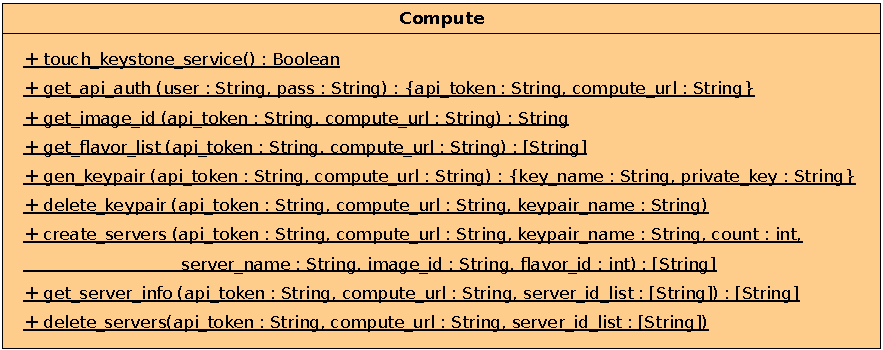
\includegraphics[width=0.99\textwidth]{imagenes/028.pdf}
 \caption{Class Diagram --- Compute module (II)}
\label{fig:diagramaclasescompute2}
\end{center}
\end{figure}

\begin{description}
 \item[List of type T:] \texttt{[T]}
 \item[Dictionary:] \texttt{\{<Key1> : <T1>, <Key2> : <T2> ... \}}
\end{description}

\subsubsection{Class Diagram --- Django and Fabric}\label{subsubsec:clasesdjangofabric}
\noindent Figure \ref{fig:djangoyfabric} exposes the relationship between the most important Django and Fabric modules.

\begin{figure}[tbp]
\begin{center}
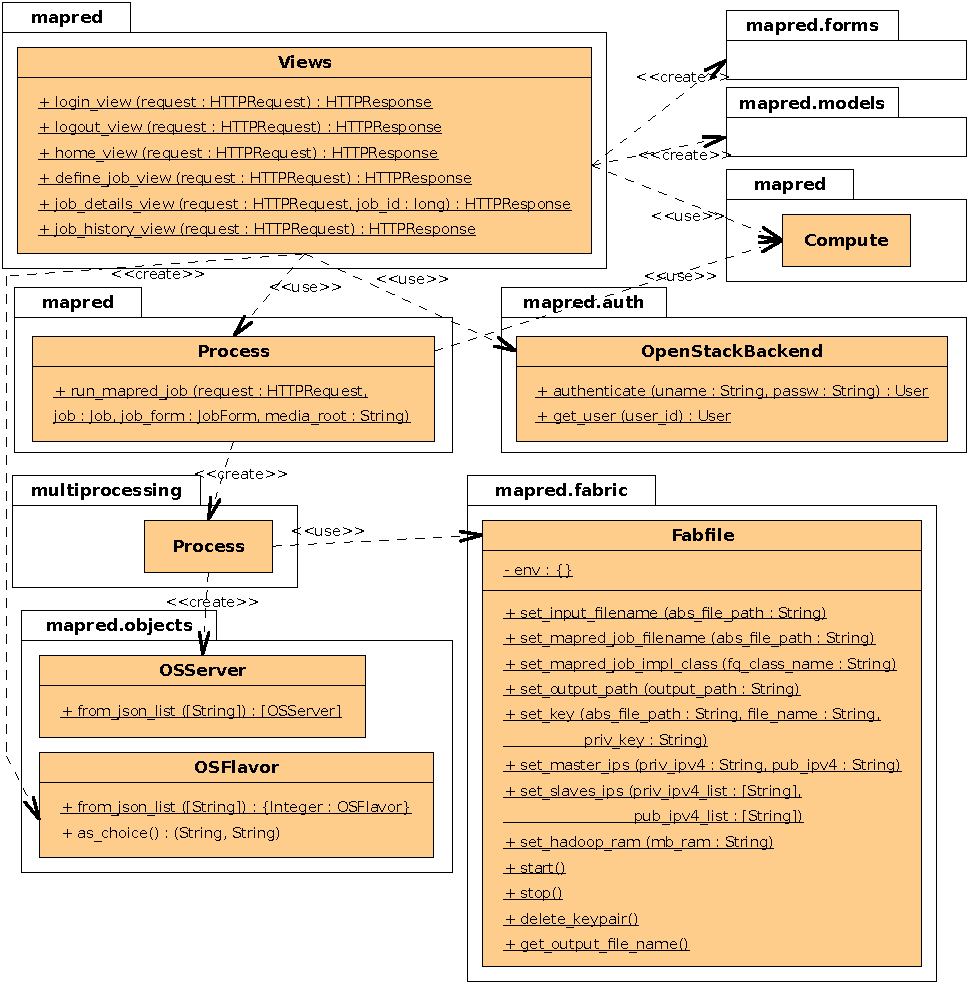
\includegraphics[width=0.99\textwidth]{imagenes/029.pdf}
 \caption{Class Diagram --- Django and Fabric}
\label{fig:djangoyfabric}
\end{center}
\end{figure}

\begin{description}
 \item[Views:] Is a delegate class implementing the behavior on each \emph{view}. It interacts with qosh Compute module to communicate with the cloud.
 \item[Process:] Is a \texttt{multiprocessing.Process} wrapper class encapsulating the logic to create processes that will handle Hadoop workflows execution collaborating with \texttt{Compute} and \texttt{Fabric} modules.
 \item[OpenStackBackend:] Is a small class that manages user logins. It is plugged into Django authenticating pipeline to delegate the clearing of user credentials to Keystone. In so doing, user access details will remain securely stored with Keystone with no need to have them duplicately stored.
 \item[OSServer y OSFlavor:] Are a kind of \emph{Transfer Object}s holding a subset of the outputted JSON data returned from the invocation of OpenStack REST API.
\end{description}

\subsubsection{Class Diagram --- Django Objects}\label{subsubsec:clasesobjetosdjango}
\noindent Figure \ref{fig:clasesobjetosdjango} details the relationships among the set of classes implementing the interaction with the web interface as provided by Django.

\begin{figure}[tbp]
\begin{center}
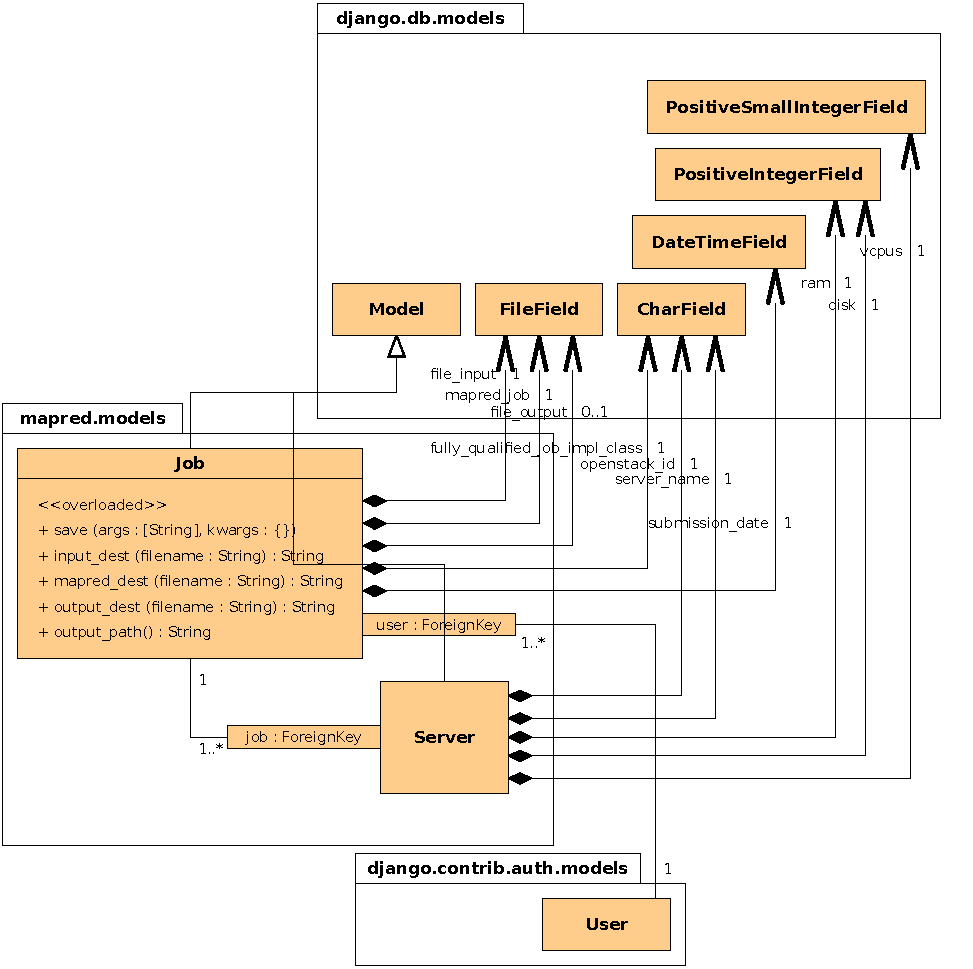
\includegraphics[width=0.99\textwidth]{imagenes/030.pdf}
 \caption{Class Diagram --- Django Objects}
\label{fig:clasesobjetosdjango}
\end{center}
\end{figure}

\begin{description}
 \item[django.db.models:] The objects defined therein model the business logic of our application. Django supplies a large set of templates that may be extended and/or composed to implement the particularities of different applications.
  \begin{description}
   \item[Model:] Is the base class of the object model supporting the business logic. Every object within the \emph{model layer} of our application extends this class --- i.e. \texttt{Job} and \texttt{Server}. Django object-relational mapper automatically translates this object model into a relational model as well as object-based queries into SQL ones.
   \item[Fields:] Hold the information related to object model classes helping Django persist the properties of the objects in a relational data base.
  \end{description}
 \item[Job:] Holds the meta-data of a Hadoop MapReduce workflow. MySQL will store these data persistently, meanwhile the file system in the Cloud Controller will actually store the information associated with the execution --- the jar file with the implementing MapReduce algorithm, inputs and outputs.
 \item[Server:] Contains the operating features of each virtual machine that had been part of a Hadoop job.
 \item[User:] Is the {Transfer Object} that is used to convey user-related information from the authorization back-end to the web interface.
\end{description}

\subsubsection{Class Diagram --- Django Forms}\label{subsubsec:clasesformulariosdjango}
\noindent Figura \ref{fig:clasesformulariosdjango} shows the class breakdown supporting the job configuration-holding forms of the web interface. \texttt{django.forms} package is laid out like the \texttt{django.db.models} package discussed above, being in this case \texttt{Form}, together with any \texttt{Field} required, the extensible class Django provides to concrete user forms.

\begin{figure}[tbp]
\begin{center}
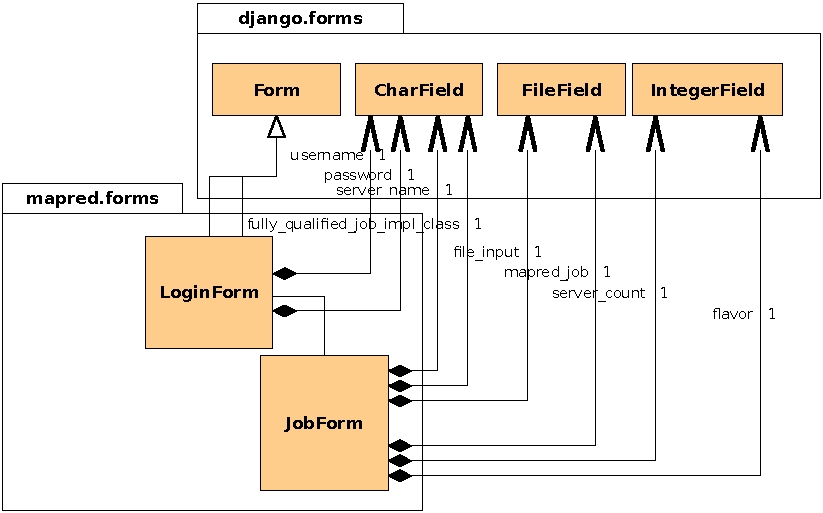
\includegraphics[width=0.99\textwidth]{imagenes/031.pdf}
 \caption{Class Diagram --- Django Forms}
\label{fig:clasesformulariosdjango}
\end{center}
\end{figure}

\begin{description}
 \item[LoginForm:] Is the user sign in form. Made up of two character fields holding the user name and password.
 \item[JobForm:] As its name suggests, is the form that allows for defining the workflow configuration. It is formed up by a set of \texttt{Fields} containing the following information: the virtual server name prefix, the qualified name of the Java class implementing the Mapper and Reducer, the input file, the \texttt{jar} package, the number of virtual servers to be deployed and their computational \emph{flavor}.
\end{description}


\subsubsection{Entity-Relationship Diagram}\label{subsubsec:entidadrelacion}
\noindent It has been pointed briefly that Django can automatically build the data base logical model derived from the object schema as written by the developer. And as expected, \emph{CRUD} operations on the DB are also managed by Django. Figure \ref{fig:entidadrelacion} shows the actual \emph{Entity-Relationship} diagram of the schema that is contained in the DB.

\begin{figure}[bp]
\begin{center}
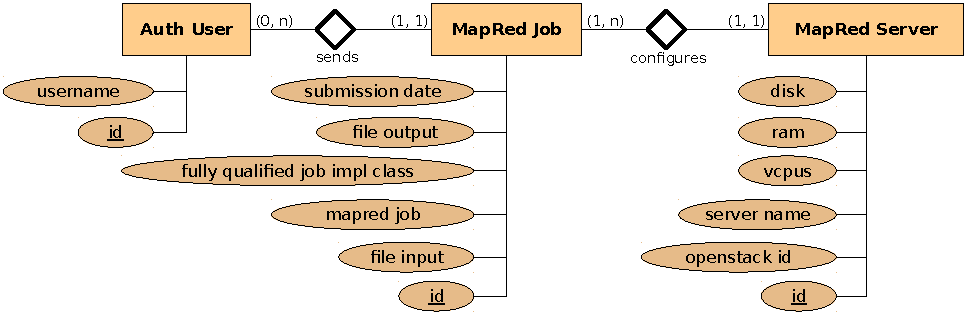
\includegraphics[width=0.99\textwidth]{imagenes/032.pdf}
 \caption{Entity-Relationship Diagram}
\label{fig:entidadrelacion}
\end{center}
\end{figure}

\subsubsection{Sequence Diagrams}\label{subsubsec:secuencia}
\noindent Figures \ref{fig:secuencia1} y \ref{fig:secuencia2} present two Sequence Diagams. They reflect the most interesting subset of messages that are interchanged between the different execution-participating entities. The sequences suppose that no errors raise during the interaction, that the user has previously signed in, that every job defining information is typed correctly and that the quota lets the deployment of the virtual cluster be carried through. Figura \ref{fig:secuencia1} pictures the full interaction. Figure \ref{fig:secuencia2} details the collaboration between classes after message \emph{\#24} in figure \ref{fig:secuencia1}.

\begin{figure}[tbp]
\begin{center}
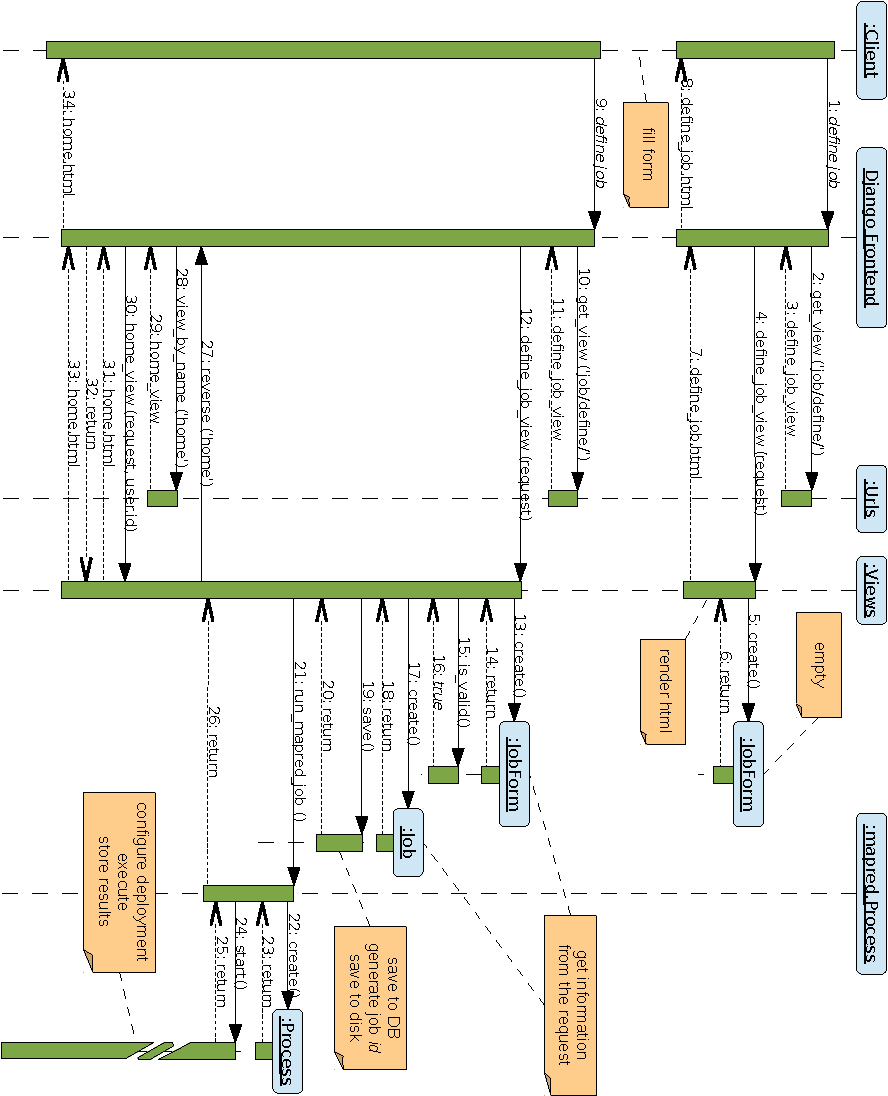
\includegraphics[width=0.99\textwidth]{imagenes/033.pdf}
 \caption{Sequence Diagram (I)}
\label{fig:secuencia1}
\end{center}
\end{figure}

\begin{figure}[tbp]
\begin{center}
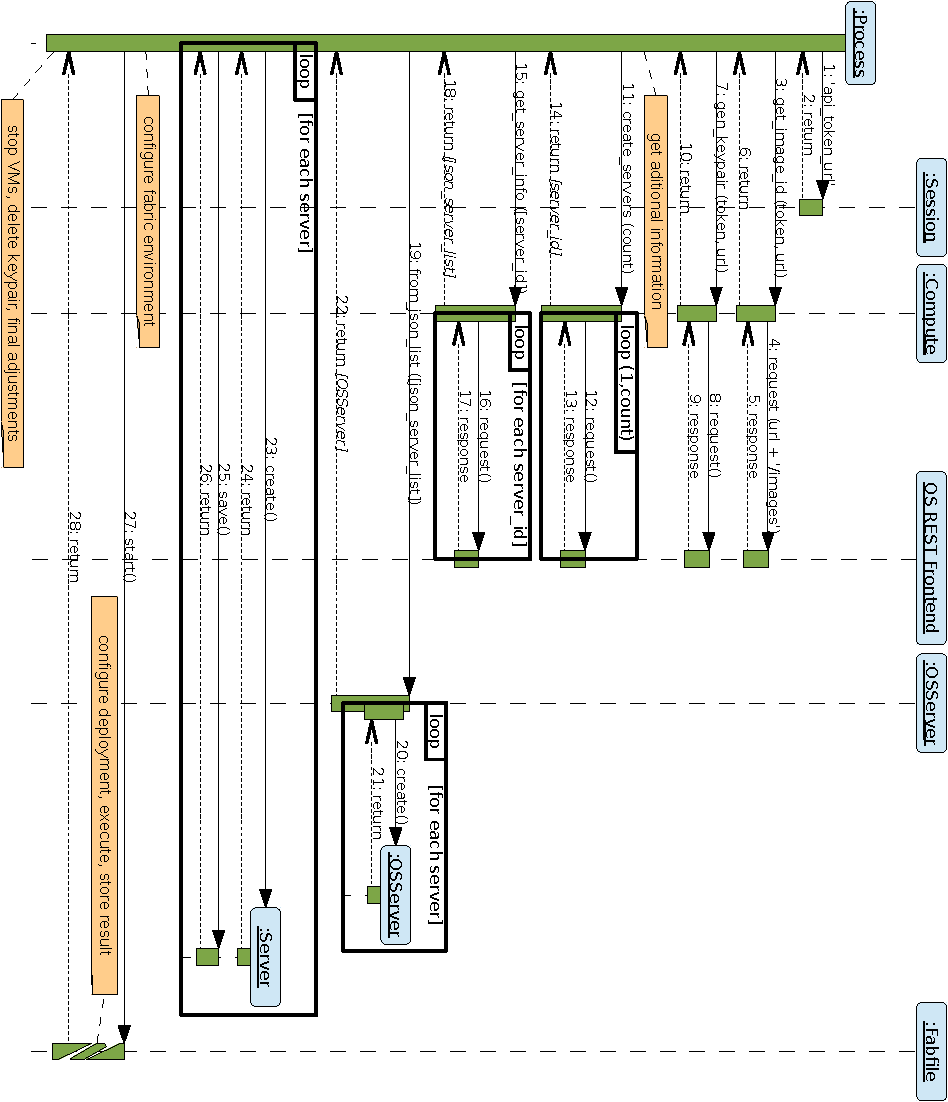
\includegraphics[width=0.99\textwidth]{imagenes/034.pdf}
 \caption{Sequence Diagram (II)}
\label{fig:secuencia2}
\end{center}
\end{figure}

